% TEMPLATE PRO PŘIDÁVÁNÍ GRAFŮ A OBRÁZKŮ DO PRÁCE
% Obsah tohoto souboru jsou příklady – nemusíš je všechny používat, ale můžeš si z nich vzít inspiraci
% POKUD SI OBSAH NEBUDEŠ JIST/Á, ZKOPÍRUJ SI PŘÍSLUŠNÝ BLOK A VLOŽ HO DO HLAVNÍHO SOUBORU

% ============================================================================
% 1. JEDNODUCHÉ VLOŽENÍ OBRÁZKU
% ============================================================================

\begin{figure}[H]
    \centering
    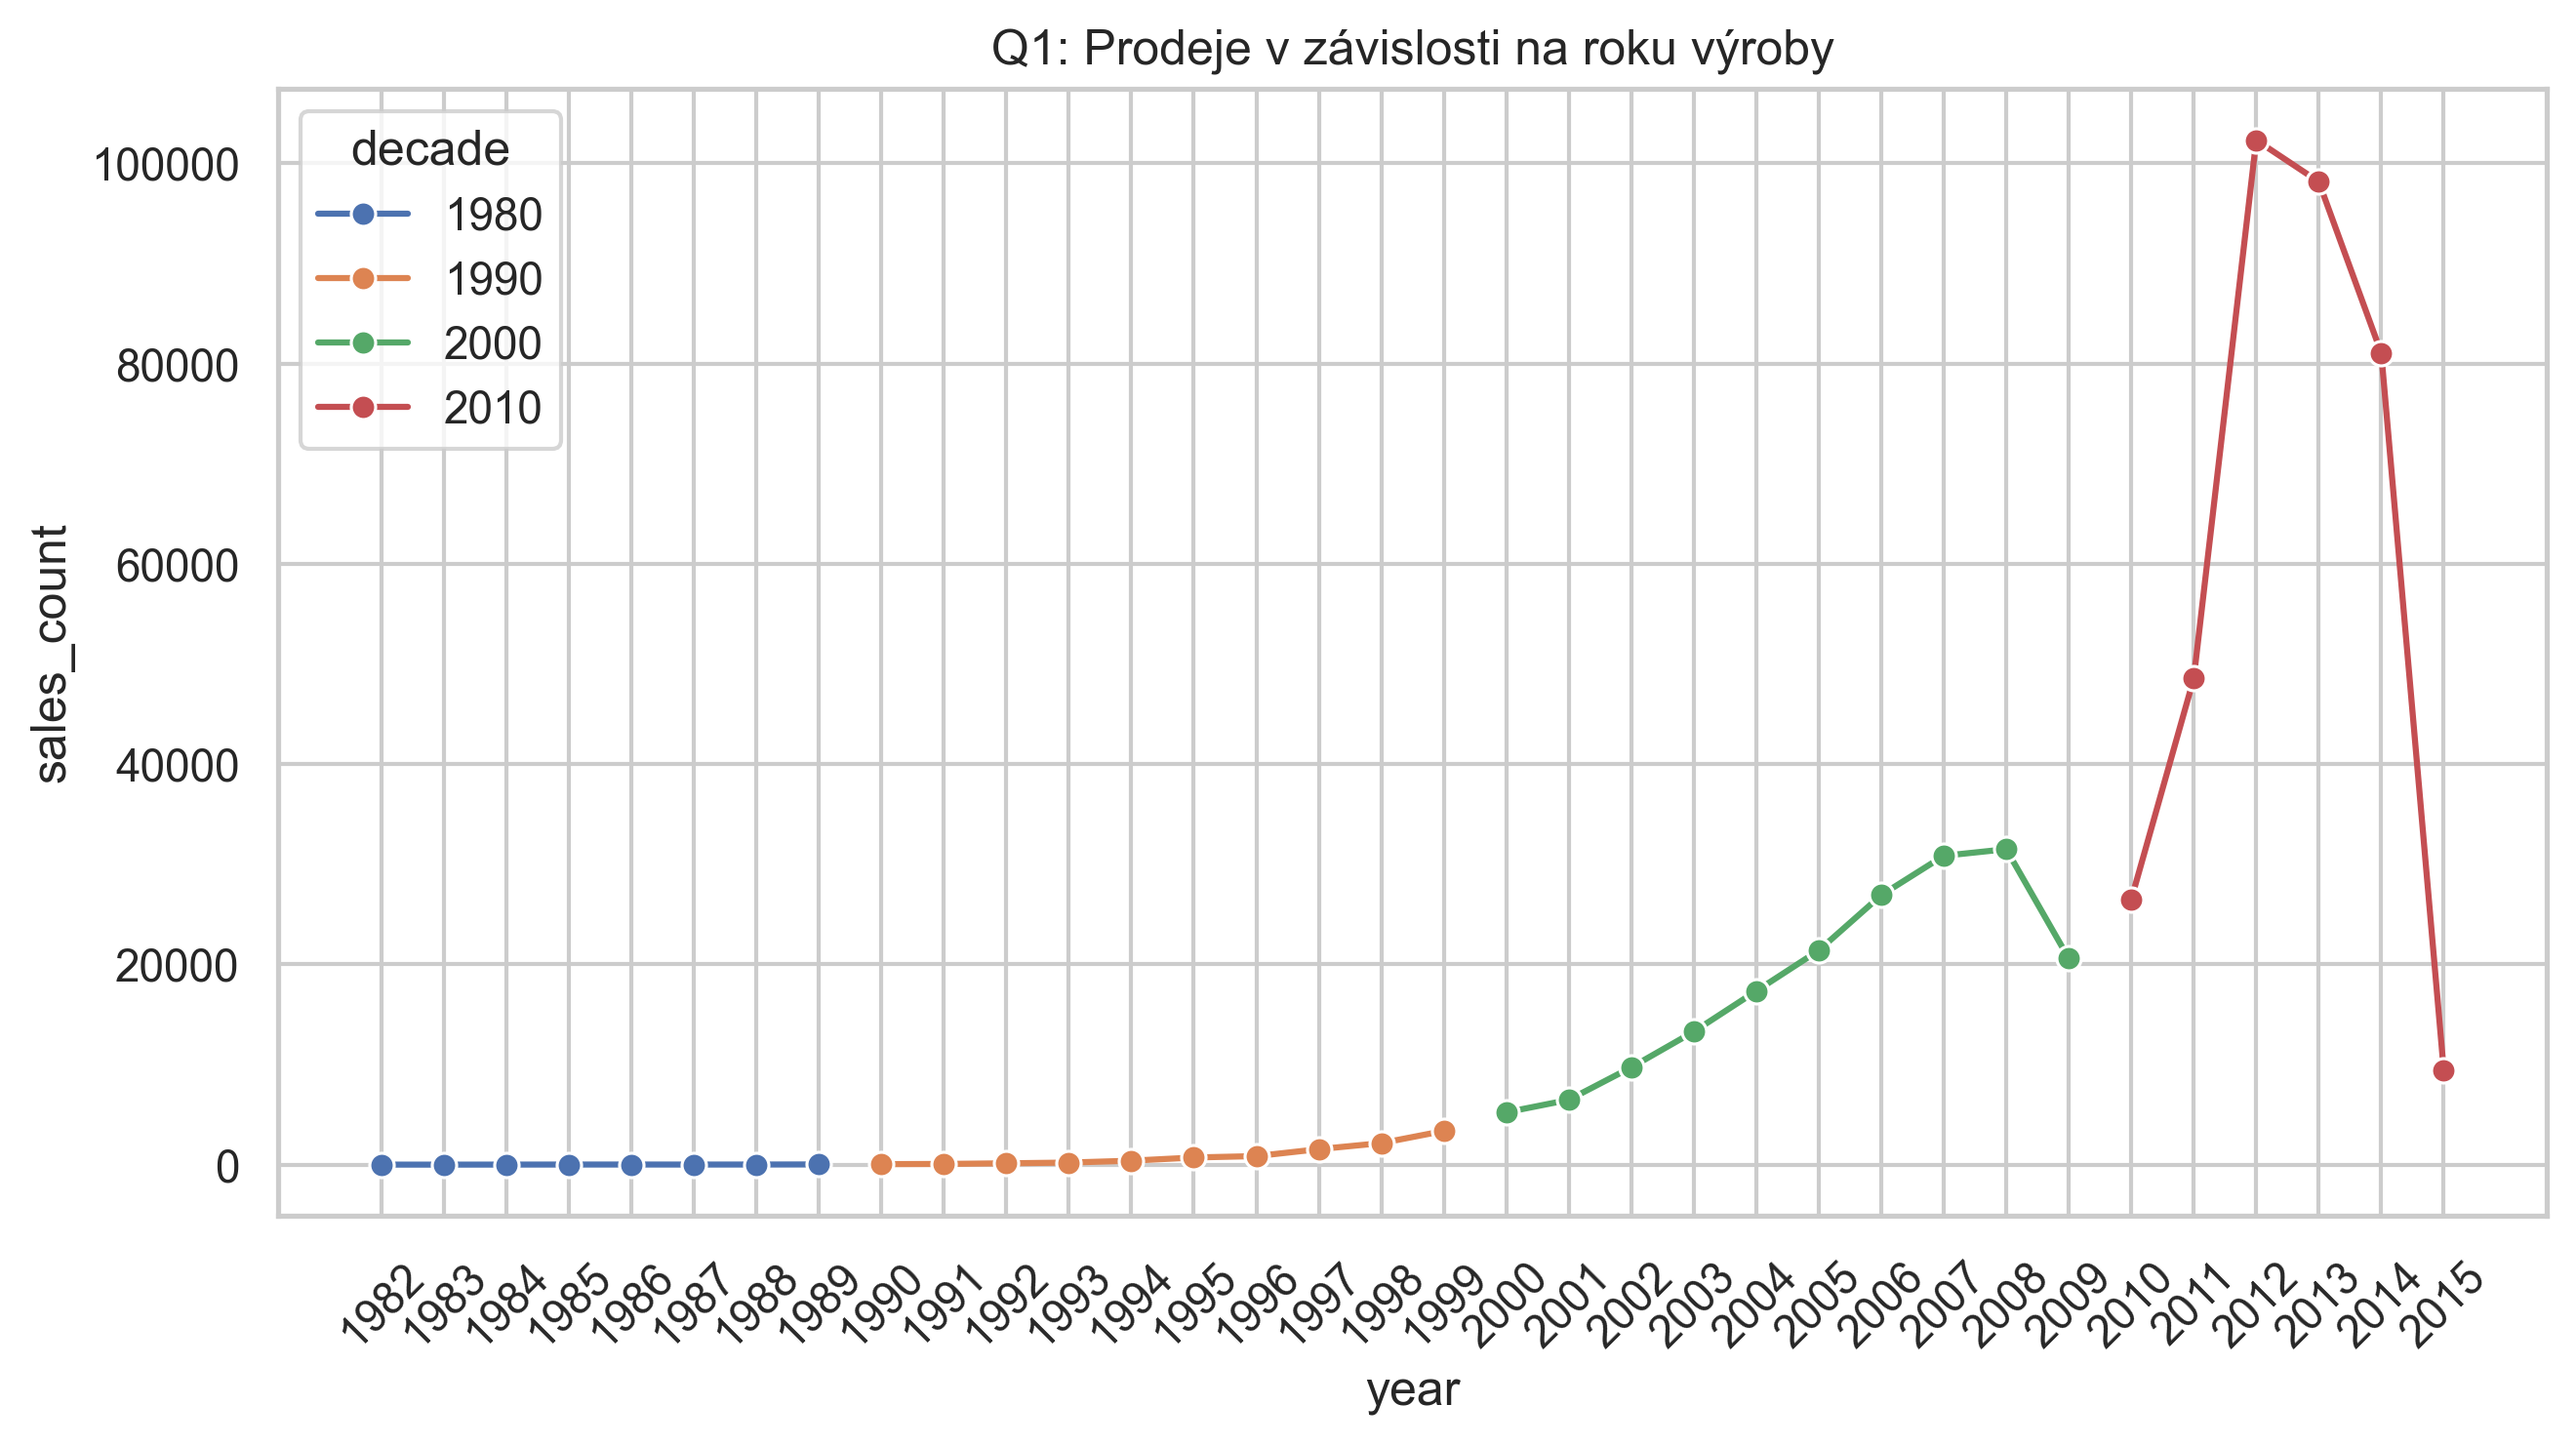
\includegraphics[width=0.85\textwidth]{../output/q1_trend.png}
    \caption{Q1: Prodeje automobilů v závislosti na roce výroby (ROLLUP hierarchie)}
    \label{fig:q1_trend}
\end{figure}

% Vysvětlení:
% - [H] = obrázek bude přesně na tomto místě (ne "floating")
% - width=0.85\textwidth = šírka 85% stránky (přizpůsob podle potřeby)
% - ../output/ = relativní cesta k obrázku (jdi o jednu úroveň výš, pak do output)
% - \caption = popis pod obrázkem (bude v seznamu obrázků)
% - \label{fig:q1_trend} = referenční značka (můžeš psát: "viz obr. \ref{fig:q1_trend}")

% ============================================================================
% 2. VLOŽENÍ GRAFU VEDLE TEXTU (DAN COLUMN LAYOUT)
% ============================================================================

\begin{wrapfigure}{r}{0.45\textwidth}
    \centering
    \includegraphics[width=0.43\textwidth]{../output/clustering_scatter.png}
    \caption{K-Means segmentace: Cena vs. Nájezd}
    \label{fig:clustering}
\end{wrapfigure}

Zde by byl text, který se obteče kolem obrázku vpravo.
To je užitečné pro krátké popisy nebo shrnutí výsledků.
Obrázek se bude zobrazovat v pravé polovině stránky.

% ============================================================================
% 3. VÍCE OBRÁZKŮ V ŘÁDKU (2x2 GRID)
% ============================================================================

\begin{figure}[H]
    \centering
    
    \begin{minipage}{0.48\textwidth}
        \centering
        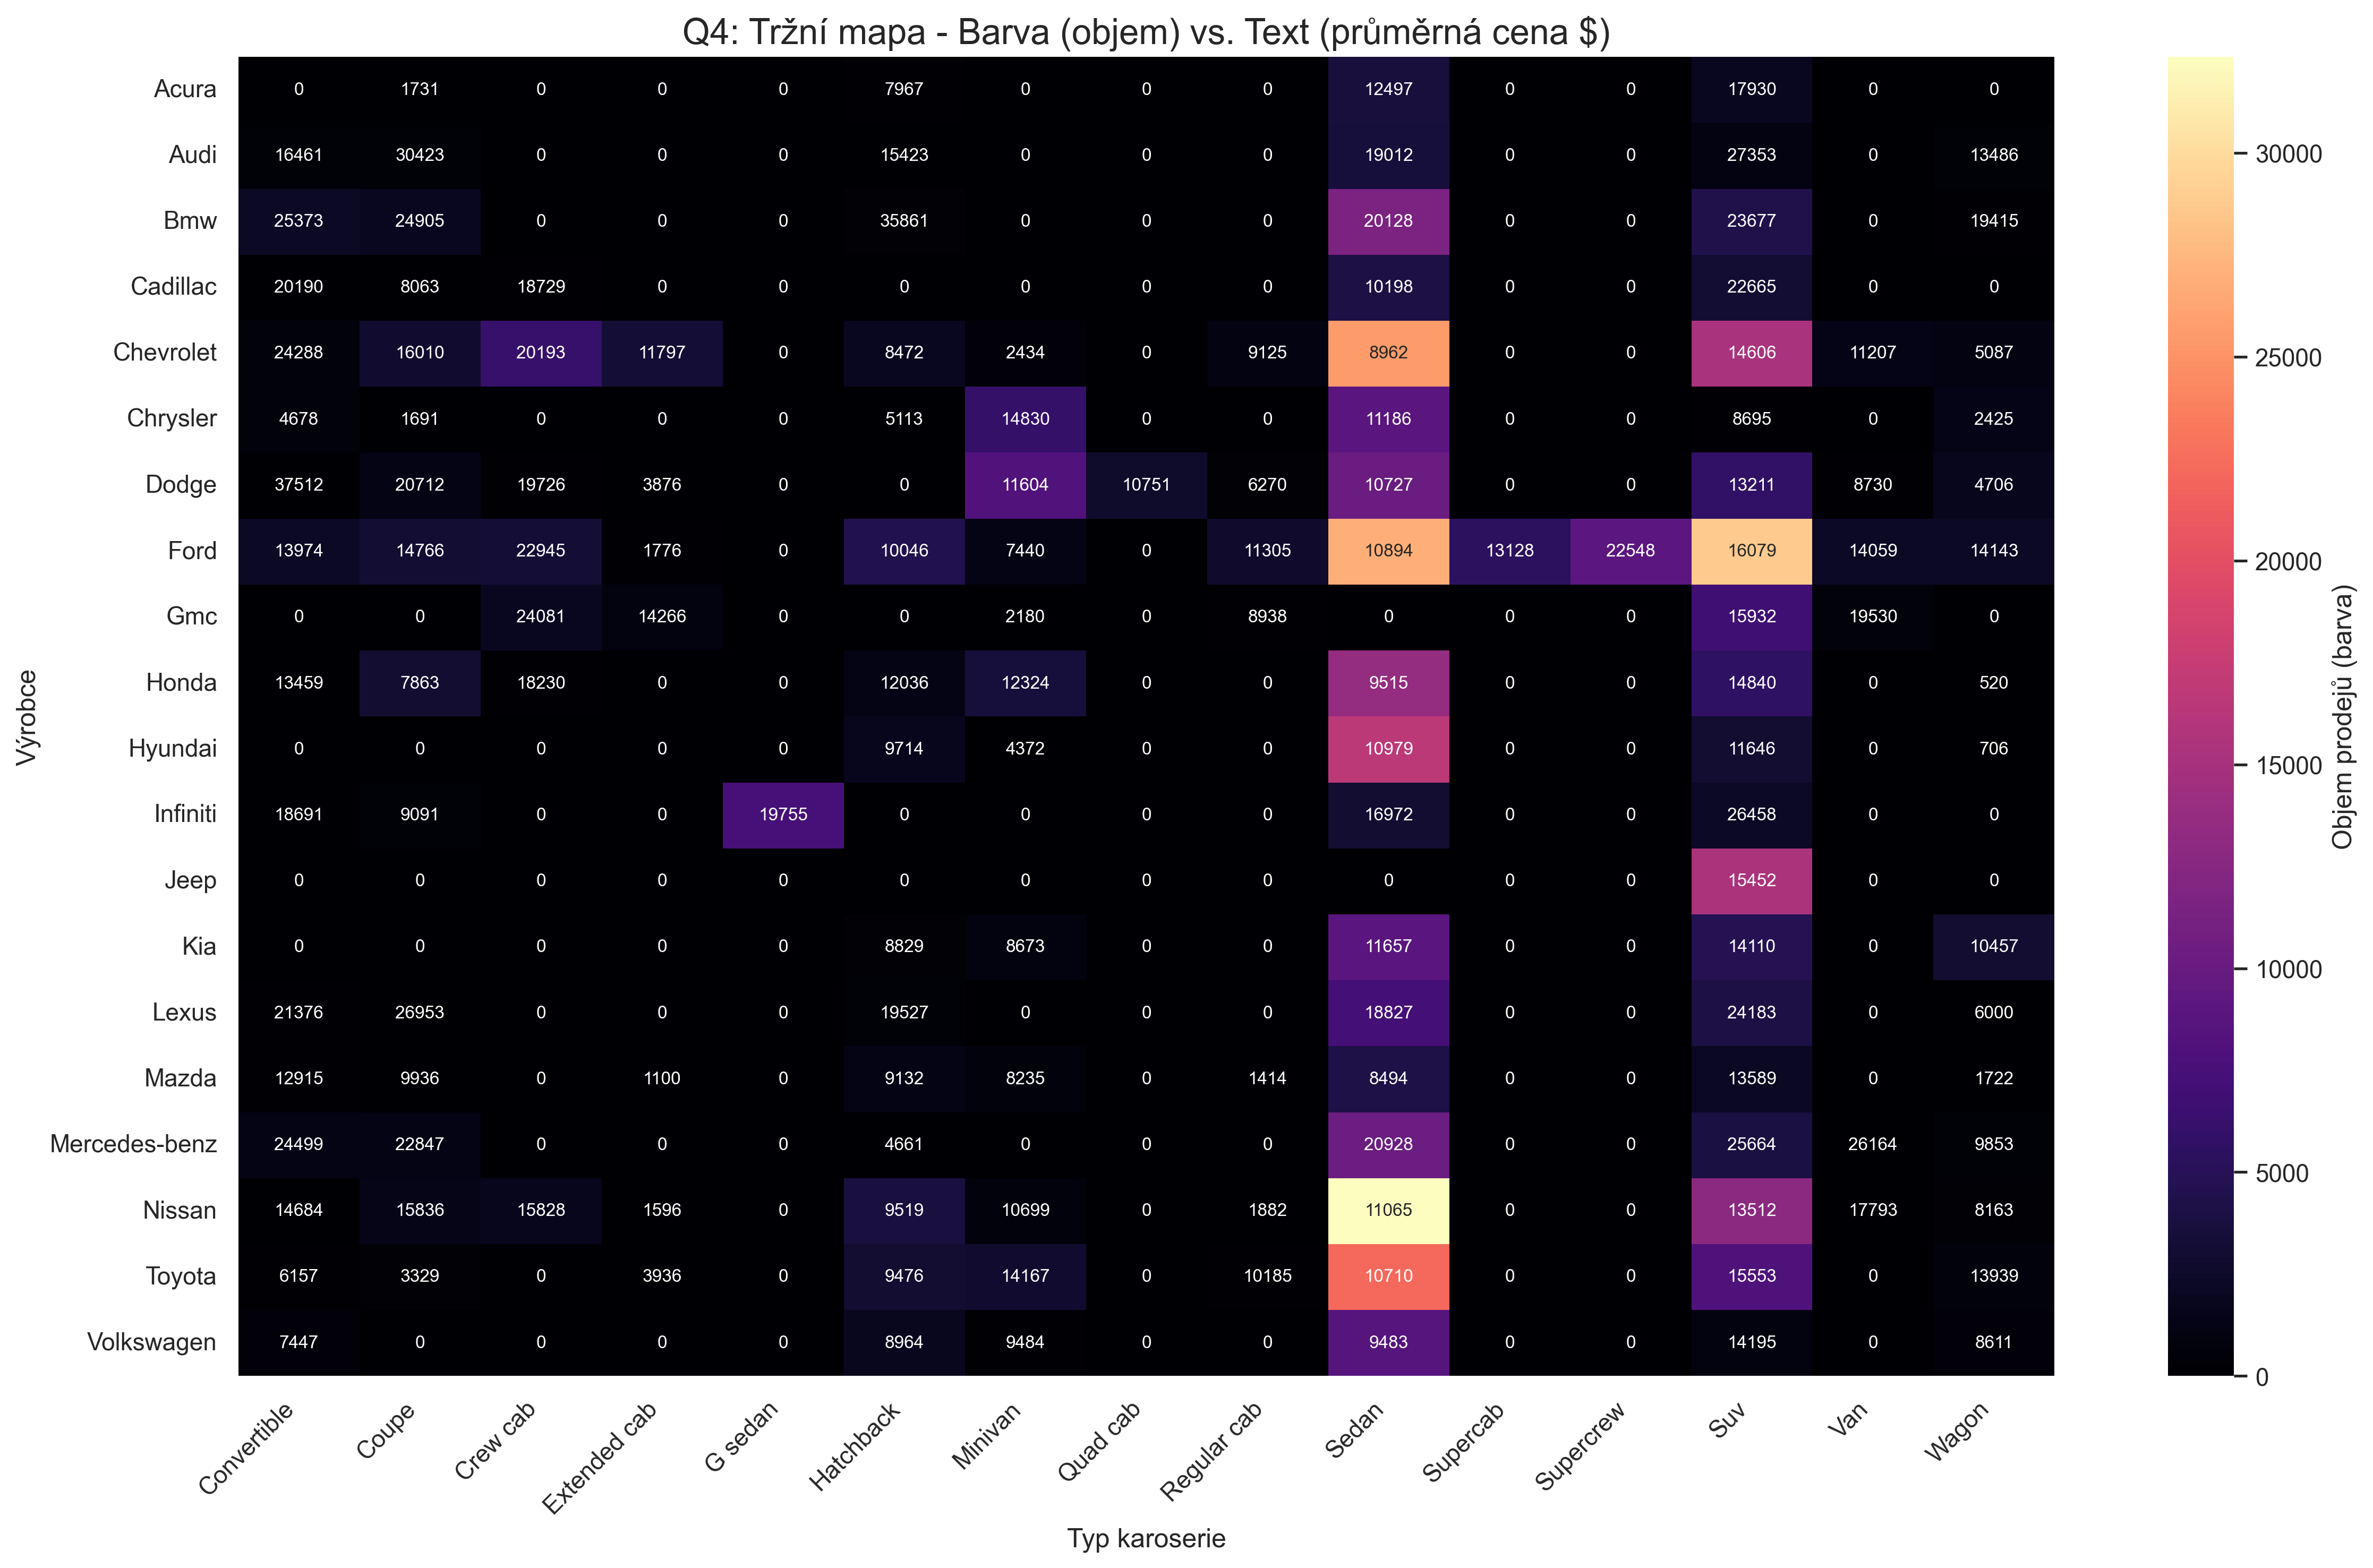
\includegraphics[width=\textwidth]{../output/q4_heatmap.png}
        \subcaption{Q4: Heatmapa Značka × Karoserie}
        \label{fig:q4a}
    \end{minipage}
    \hfill
    \begin{minipage}{0.48\textwidth}
        \centering
        \includegraphics[width=\textwidth]{../output/q5_segments.png}
        \subcaption{Q5: Segmentační matice}
        \label{fig:q5a}
    \end{minipage}
    
    \begin{minipage}{0.48\textwidth}
        \centering
        \includegraphics[width=\textwidth]{../output/benchmark_bars.png}
        \subcaption{Benchmark: DuckDB vs PostgreSQL}
        \label{fig:bench}
    \end{minipage}
    \hfill
    \begin{minipage}{0.48\textwidth}
        \centering
        \includegraphics[width=\textwidth]{../output/regression.png}
        \subcaption{Regresní trend ceny vs. rok}
        \label{fig:regression}
    \end{minipage}
    
    \caption{Přehled klíčových vizualizací}
    \label{fig:overview}
\end{figure}

% ============================================================================
% 4. OBRÁZEK S RÁMEČKEM A STÍNEM
% ============================================================================

\begin{figure}[H]
    \centering
    \fbox{
        \includegraphics[width=0.8\textwidth]{../output/important_chart.png}
    }
    \caption{Důležitý graf vyznačený rámečkem}
    \label{fig:important}
\end{figure}

% ============================================================================
% 5. VLOŽENÍ PDF SVG - POKUD MÁŠVECTOROVÉ GRAFIKY
% ============================================================================

% Pokud exportuješ z Pythonu jako PDF nebo SVG, stejně funguje:
\begin{figure}[H]
    \centering
    \includegraphics[width=0.9\textwidth]{../output/vectorized_chart.pdf}
    \caption{Vektorizovaný graf (PDF nebo SVG)}
    \label{fig:vector}
\end{figure}

% ============================================================================
% 6. DYNAMICKÁ TABULKA VEDLE GRAFU
% ============================================================================

\begin{table}[H]
    \centering
    \begin{minipage}{0.45\textwidth}
        \centering
        \caption{Statické metriky}
        \begin{tabular}{|l|r|}
            \hline
            \textbf{Metrika} & \textbf{Hodnota} \\
            \hline
            Silhouette Score & 0.72 \\
            Davies-Bouldin Index & 0.58 \\
            Clusters & 4 \\
            \hline
        \end{tabular}
    \end{minipage}
    \hfill
    \begin{minipage}{0.45\textwidth}
        \centering
        \includegraphics[width=\textwidth]{../output/elbow_method.png}
    \end{minipage}
\end{table}

% ============================================================================
% 7. PODMÍNKA: OBRÁZEK BEZ CHYBY, POKUD SOUBOR NEEXISTUJE
% ============================================================================

% Pokud chceš aby se LaTeX kompiloval i když chybí obrázek:
% Odkomentuj tento package v preambulovém kódu hlavního .tex:
% \usepackage{graphicx}

% A pak použij:
\ifpdf
    \begin{figure}[H]
        \centering
        \includegraphics[width=0.8\textwidth]{../output/maybe_missing.png}
        \caption{Obrázek, který možná neexistuje}
    \end{figure}
\else
    \textit{[Obrázek není k dispozici]}
\fi

% ============================================================================
% 8. LEGENDA PRO VÍCE OBRÁZKŮ (POKUD JSOU VÁZANÉ DOHROMADY)
% ============================================================================

\begin{figure}[H]
    \centering
    \includegraphics[width=0.85\textwidth]{../output/q2_cube_analysis.png}\\[0.3cm]
    
    \small
    \textbf{Legenda:} Barva = typ karoserie (Sedan=modrá, SUV=zelená, Truck=červená).
    Výška sloupce = počet prodejů. Číslo = průměrná cena USD.
    \label{fig:q2_legend}
\end{figure}

% ============================================================================
% 9. POZNÁMKA: POVINNÉ BALÍČKY V PREAMBULOVÉM KÓDU
% ============================================================================

% Aby všechny výše uvedené commands fungovaly, potřebuješ v preambulovém kódu (na vrcholu .tex):

% \usepackage{graphicx}        % pro \includegraphics
% \usepackage{float}           % pro [H] (exact positioning)
% \usepackage{wrapfig}         % pro \wrapfigure (text kolem obrázku)
% \usepackage{caption}         % pro \caption
% \usepackage{subcaption}      % pro \subcaption (sub-obrázky)
% \usepackage[demo]{graphicx}  % pro chybějící obrázky (demo mód)

% Všechny tyto jsou již zahrnuty v GOLAP_seminární_práce.tex, takže by mělo být OK!

% ============================================================================
% 10. PŘÍKLADY UMÍSTĚNÍ V HLAVNÍM DOKUMENTU
% ============================================================================

% V sekci "6.1 Q1: Hierarchie":
%    // po SQL kódu
%    \begin{figure}[H]
%        \centering
%        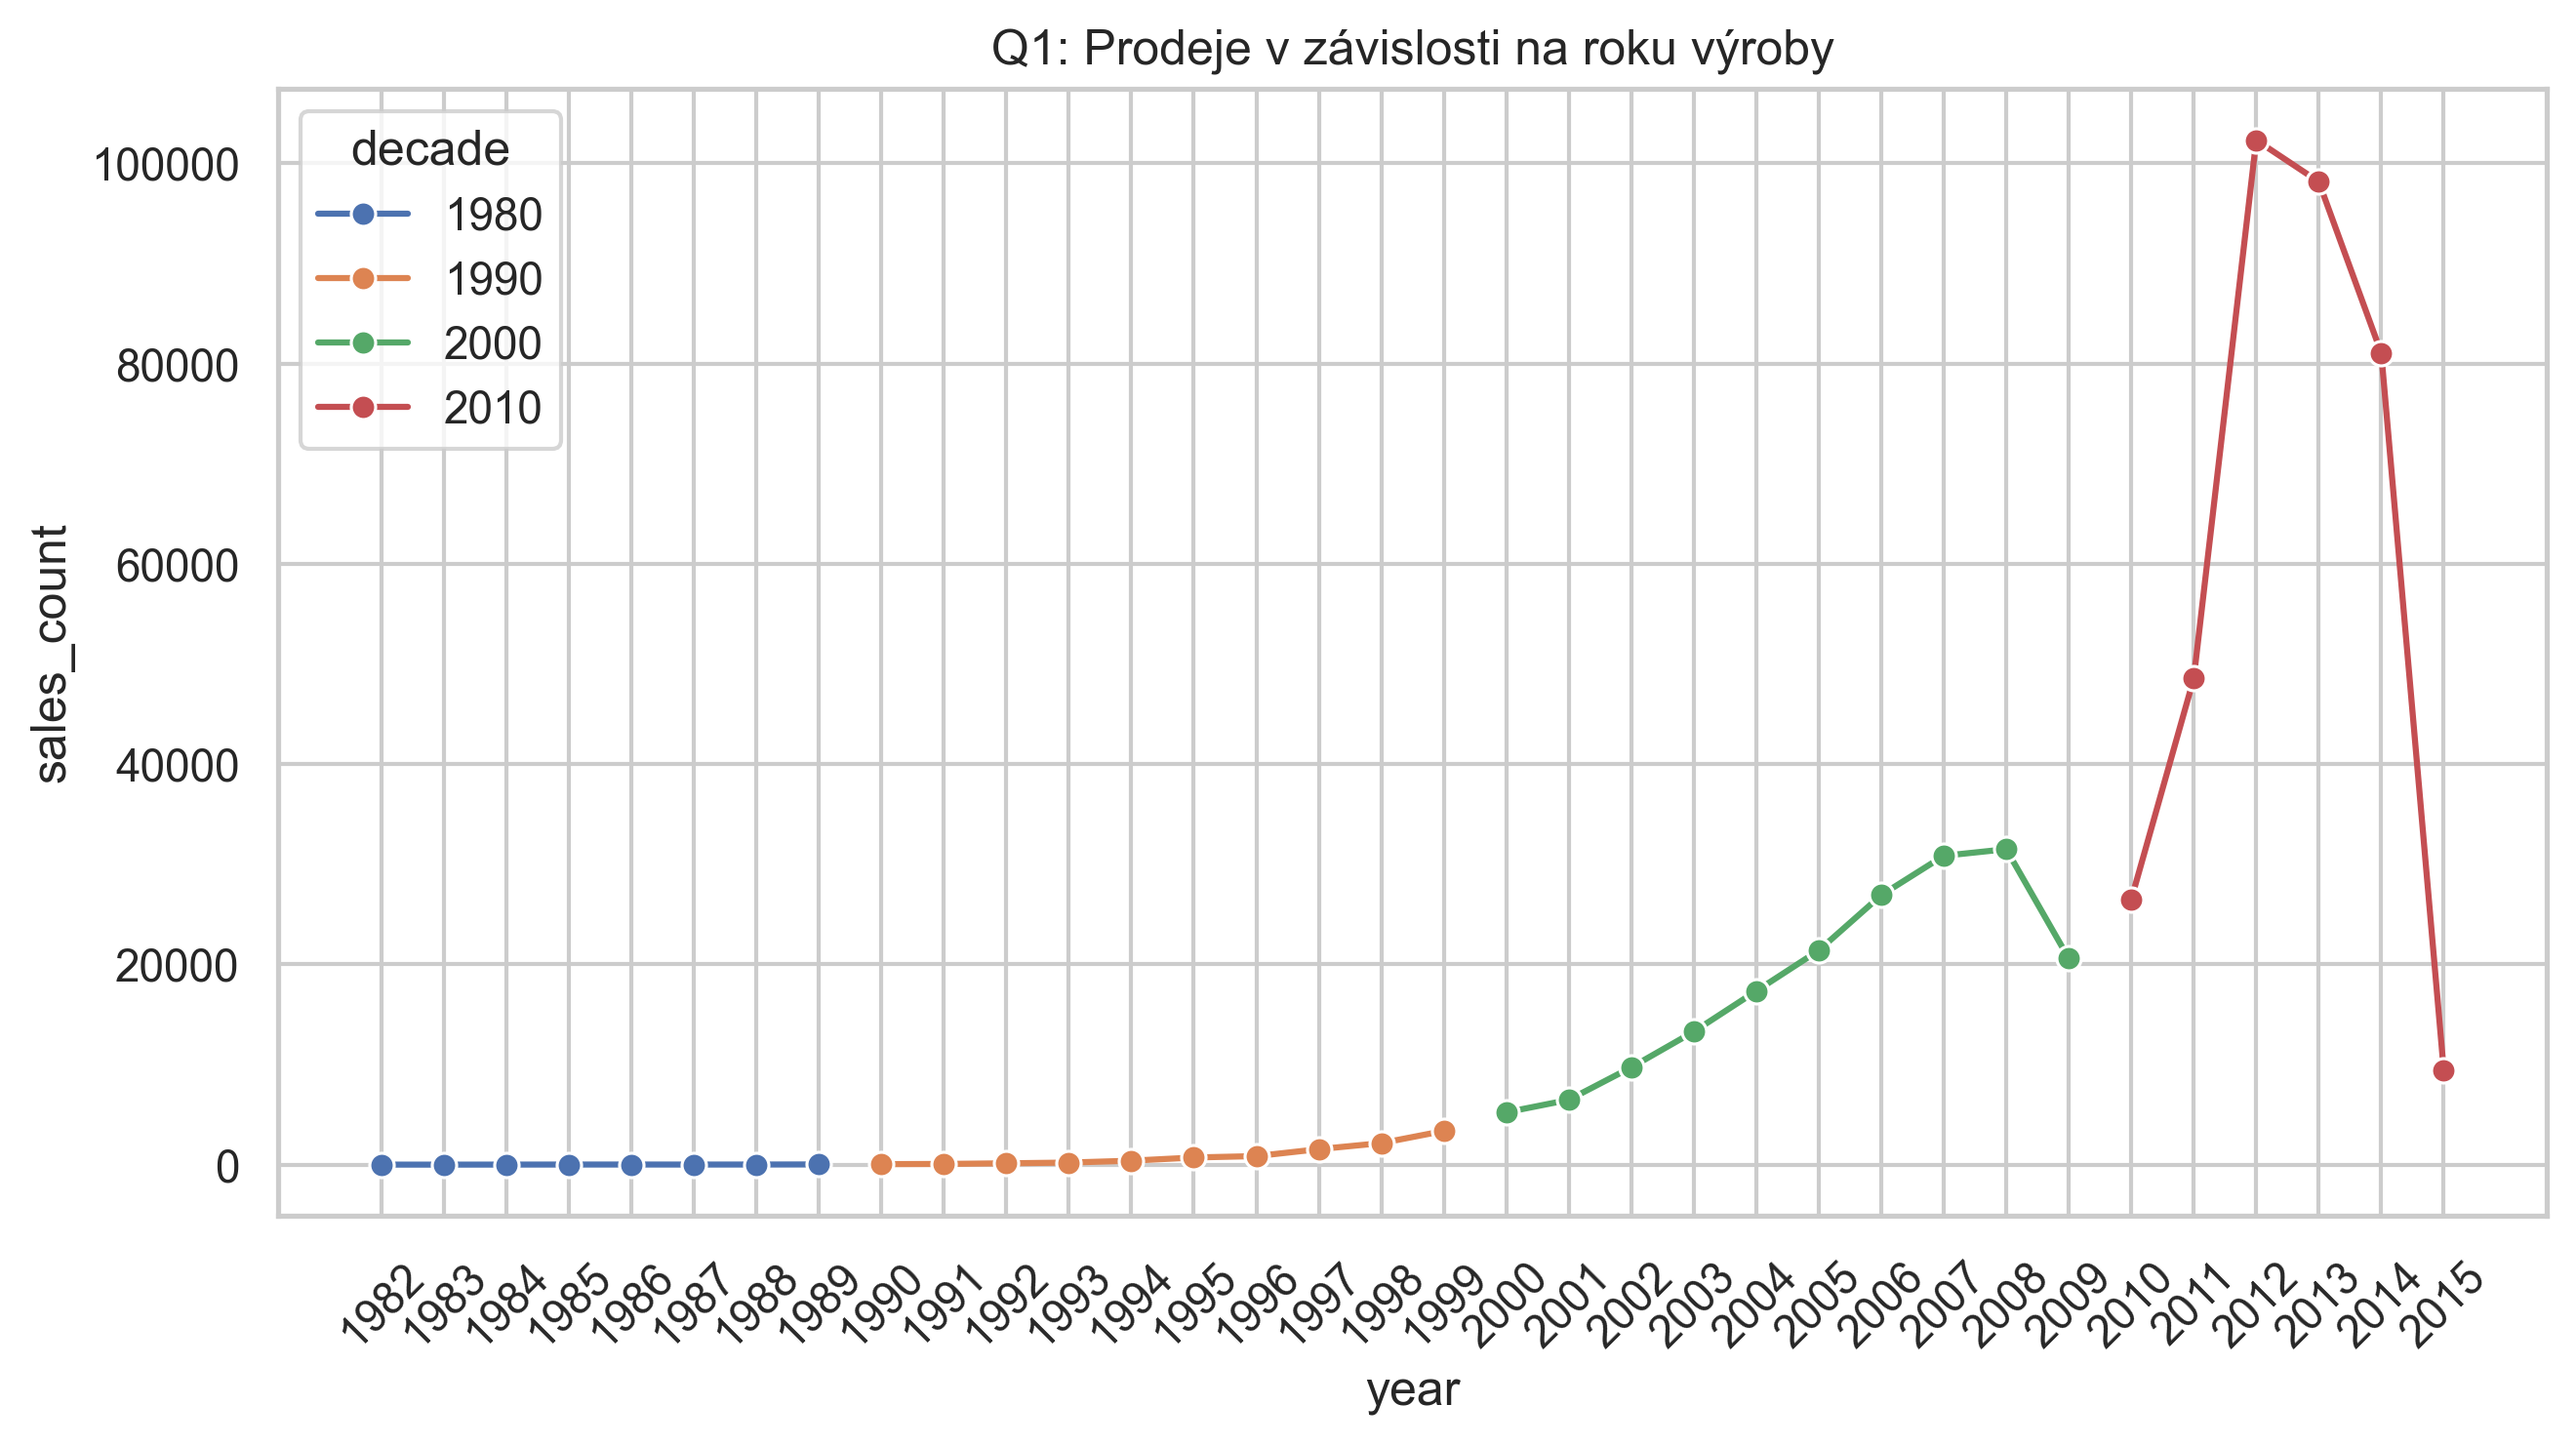
\includegraphics[width=0.85\textwidth]{../output/q1_trend.png}
%        \caption{Q1: Prodeje v čase}
%    \end{figure}

% V sekci "6.2 Q2: CUBE":
%    // po tabulce
%    \begin{figure}[H]
%        \centering
%        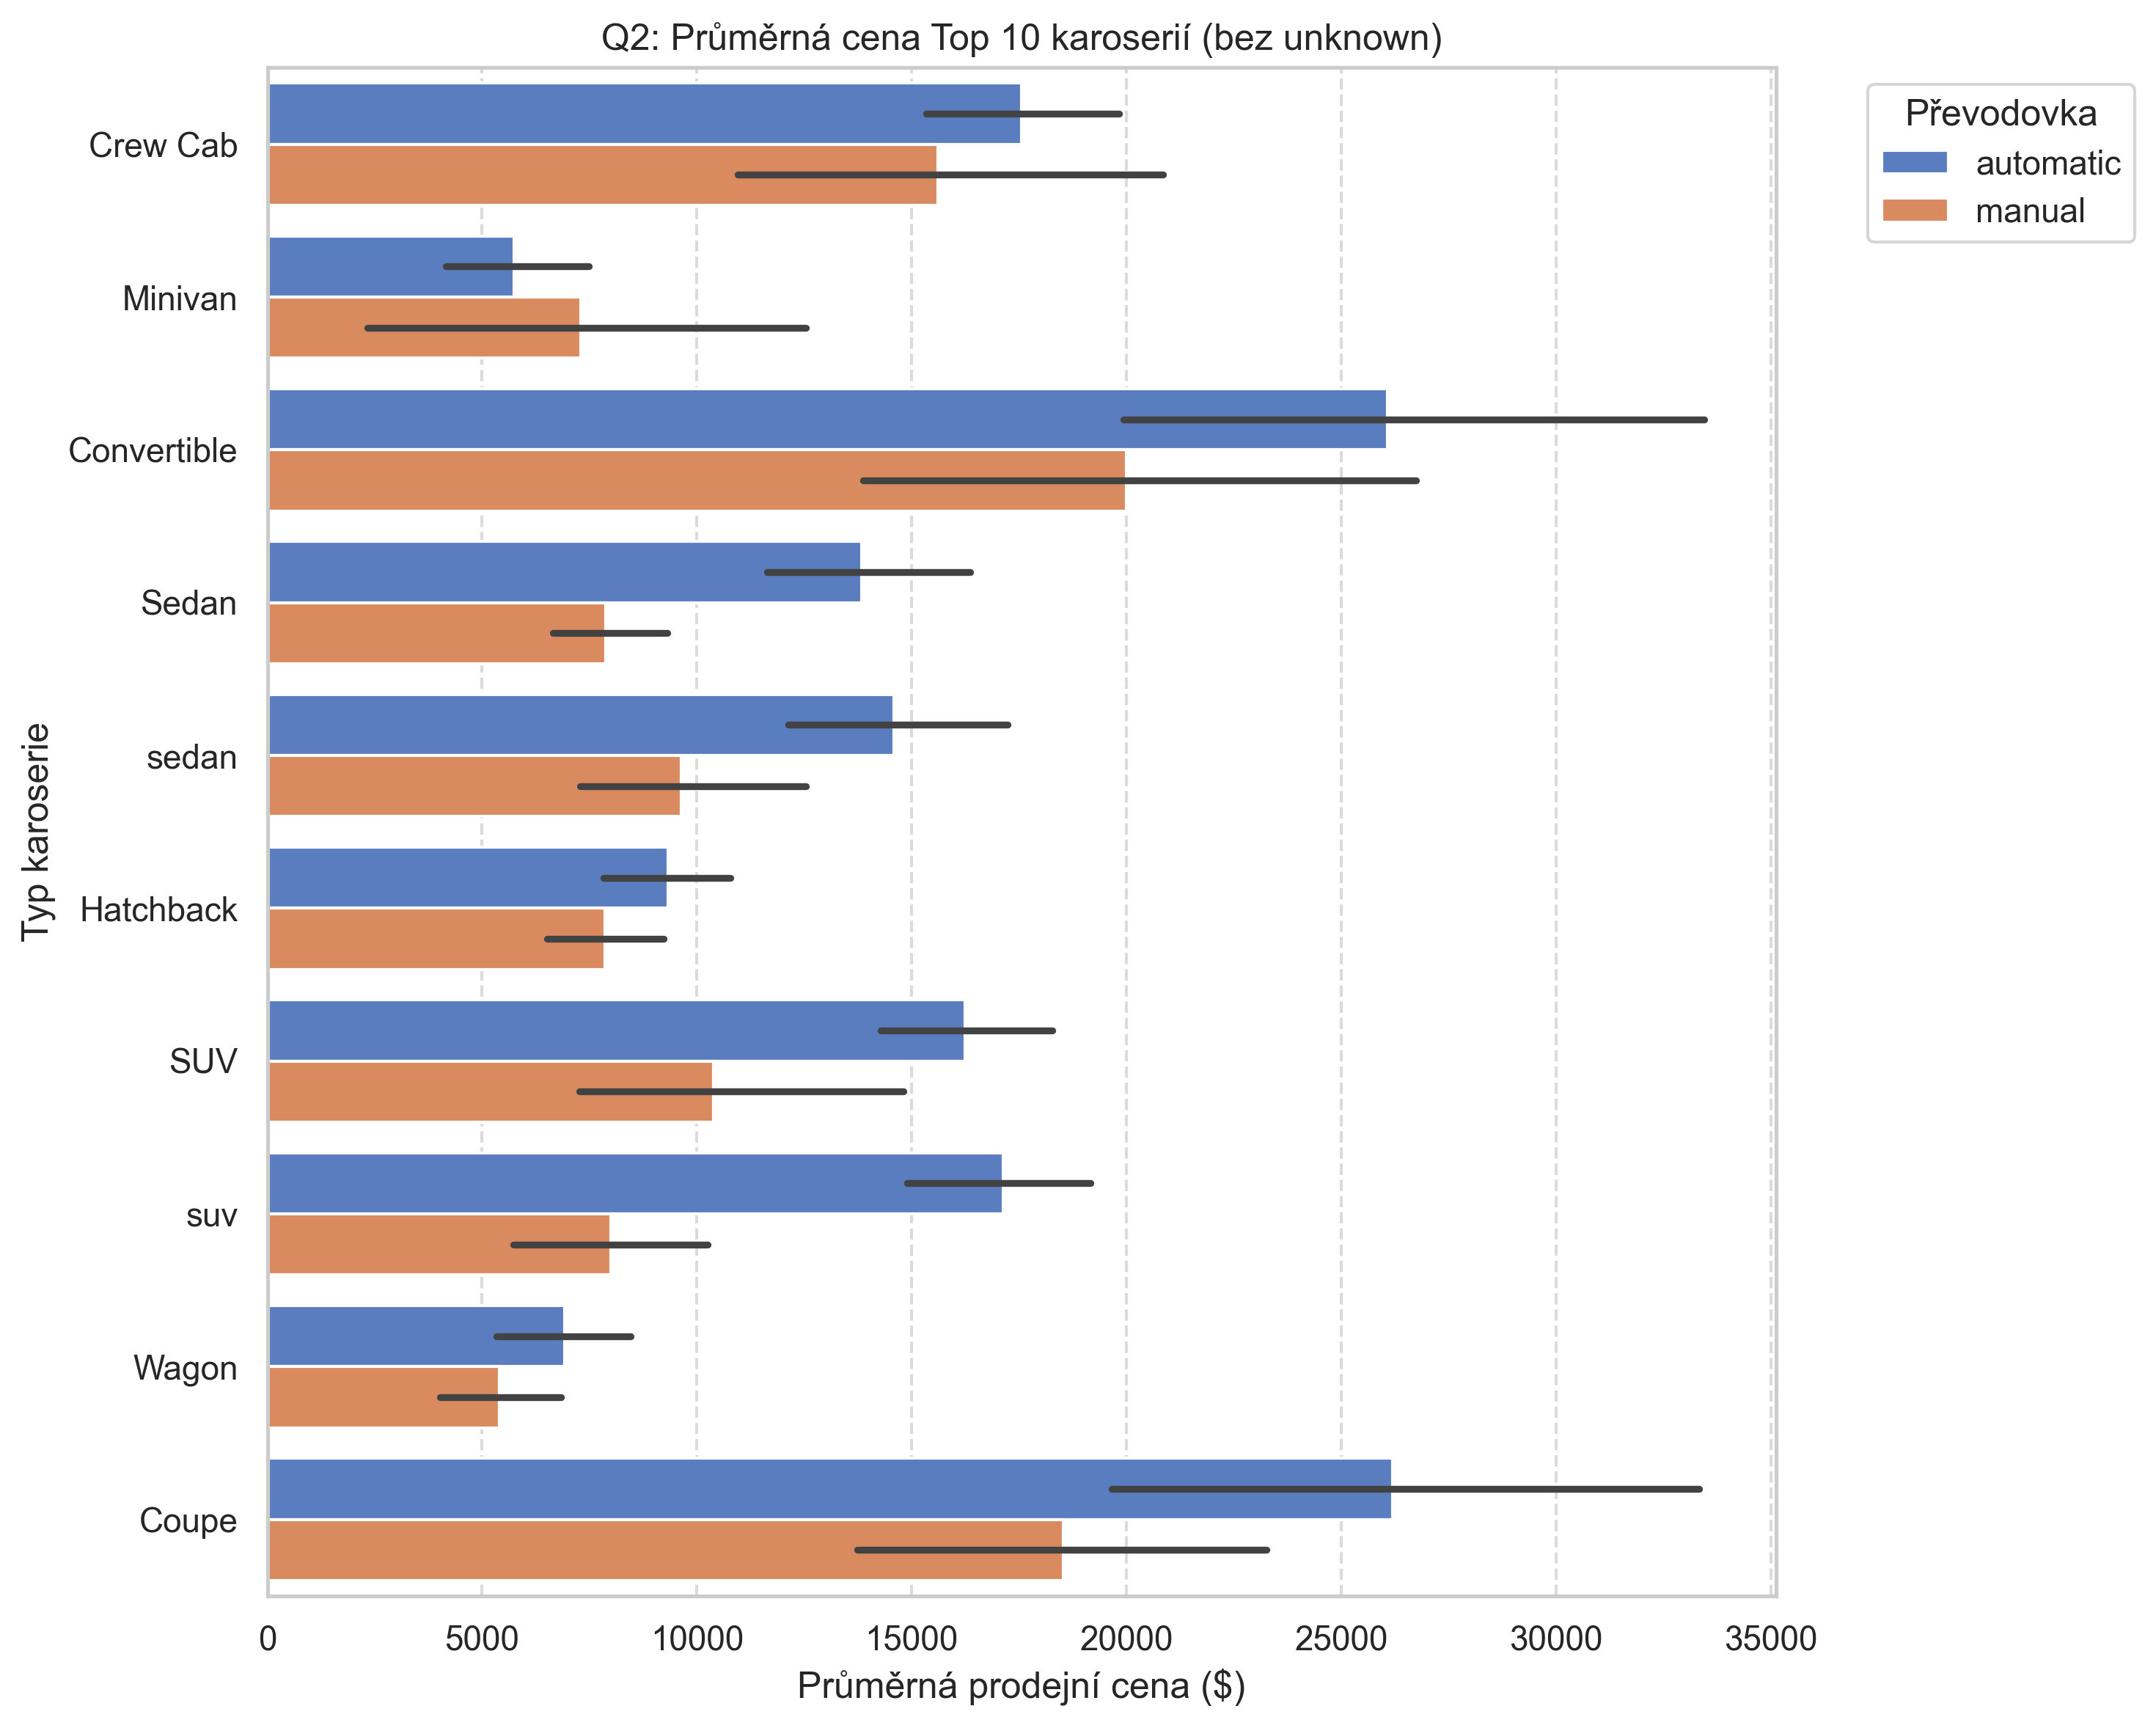
\includegraphics[width=0.85\textwidth]{../output/q2_cube_barplot.png}
%        \caption{Q2: Top 10 karoserií}
%    \end{figure}

% V sekci "7. Benchmark výsledků":
%    \begin{figure}[H]
%        \centering
%        \includegraphics[width=0.9\textwidth]{../output/benchmark_comparison.png}
%        \caption{Srovnění časů DuckDB vs PostgreSQL}
%    \end{figure}

% V sekci "8. Data Mining - A. Clustering":
%    \begin{figure}[H]
%        \centering
%        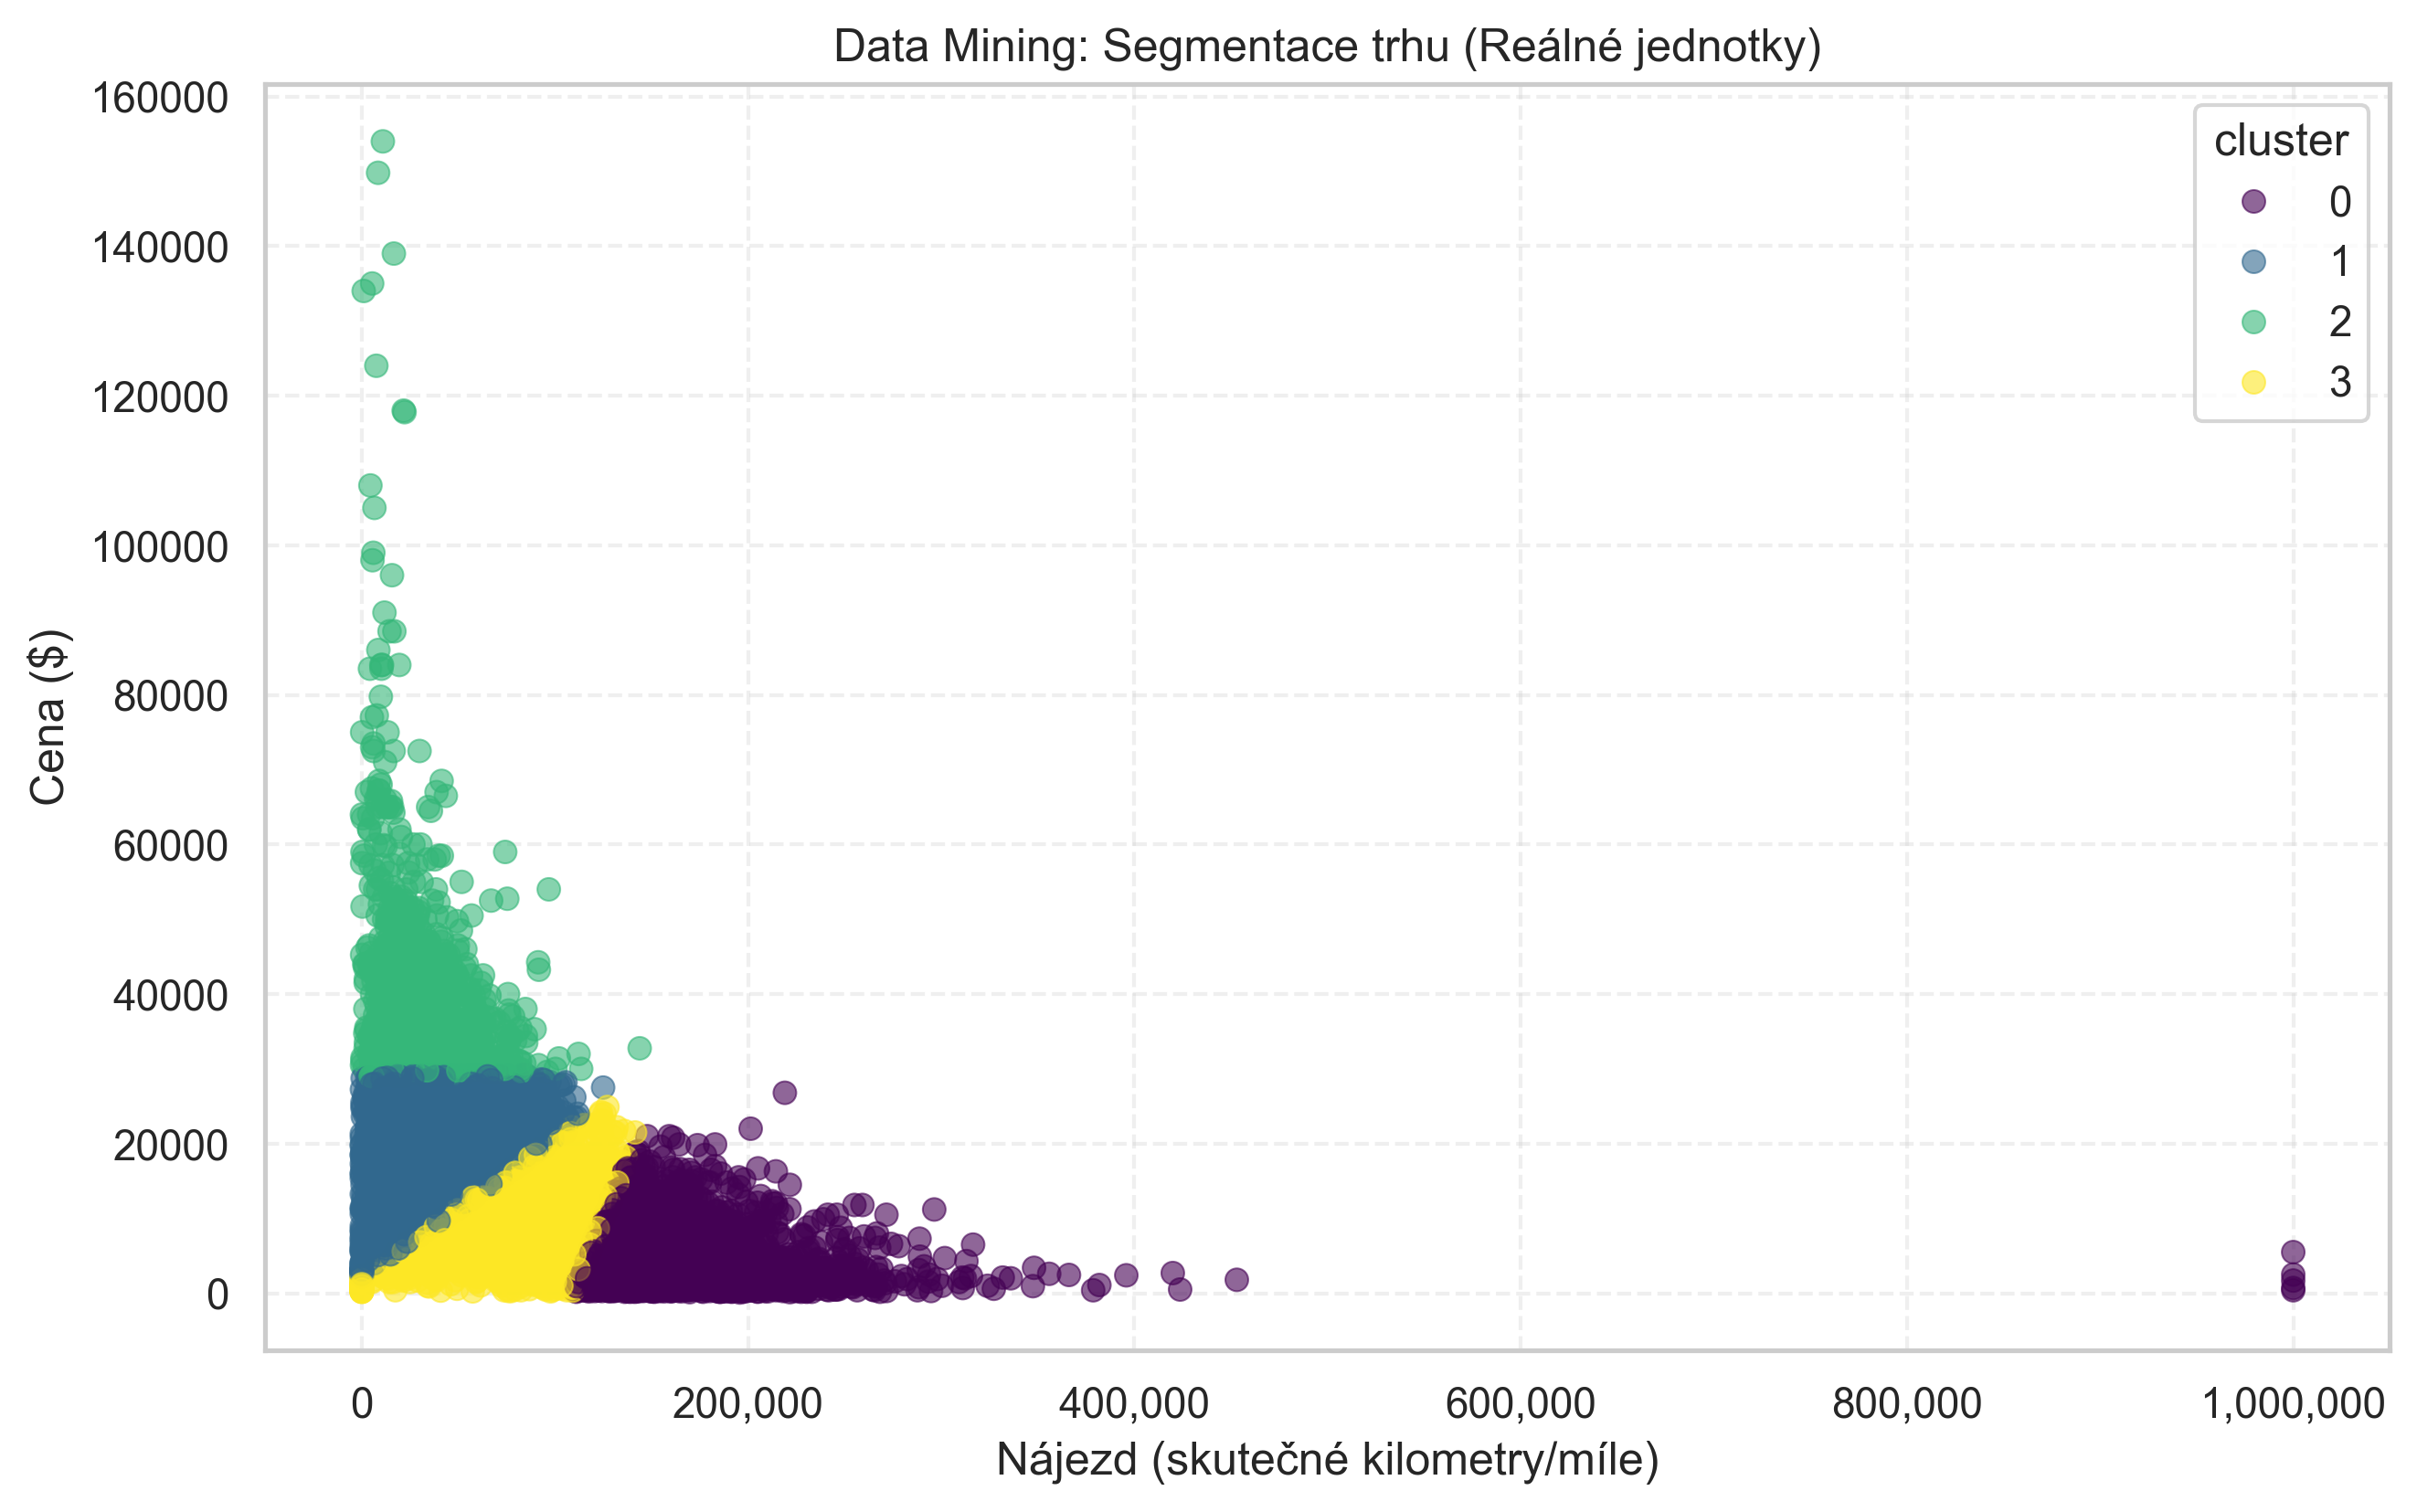
\includegraphics[width=0.8\textwidth]{../output/kmeans_scatter.png}
%        \caption{K-Means segmentace (Cena vs. Nájezd)}
%    \end{figure}

% V sekci "8. Data Mining - B. Regrese":
%    \begin{figure}[H]
%        \centering
%        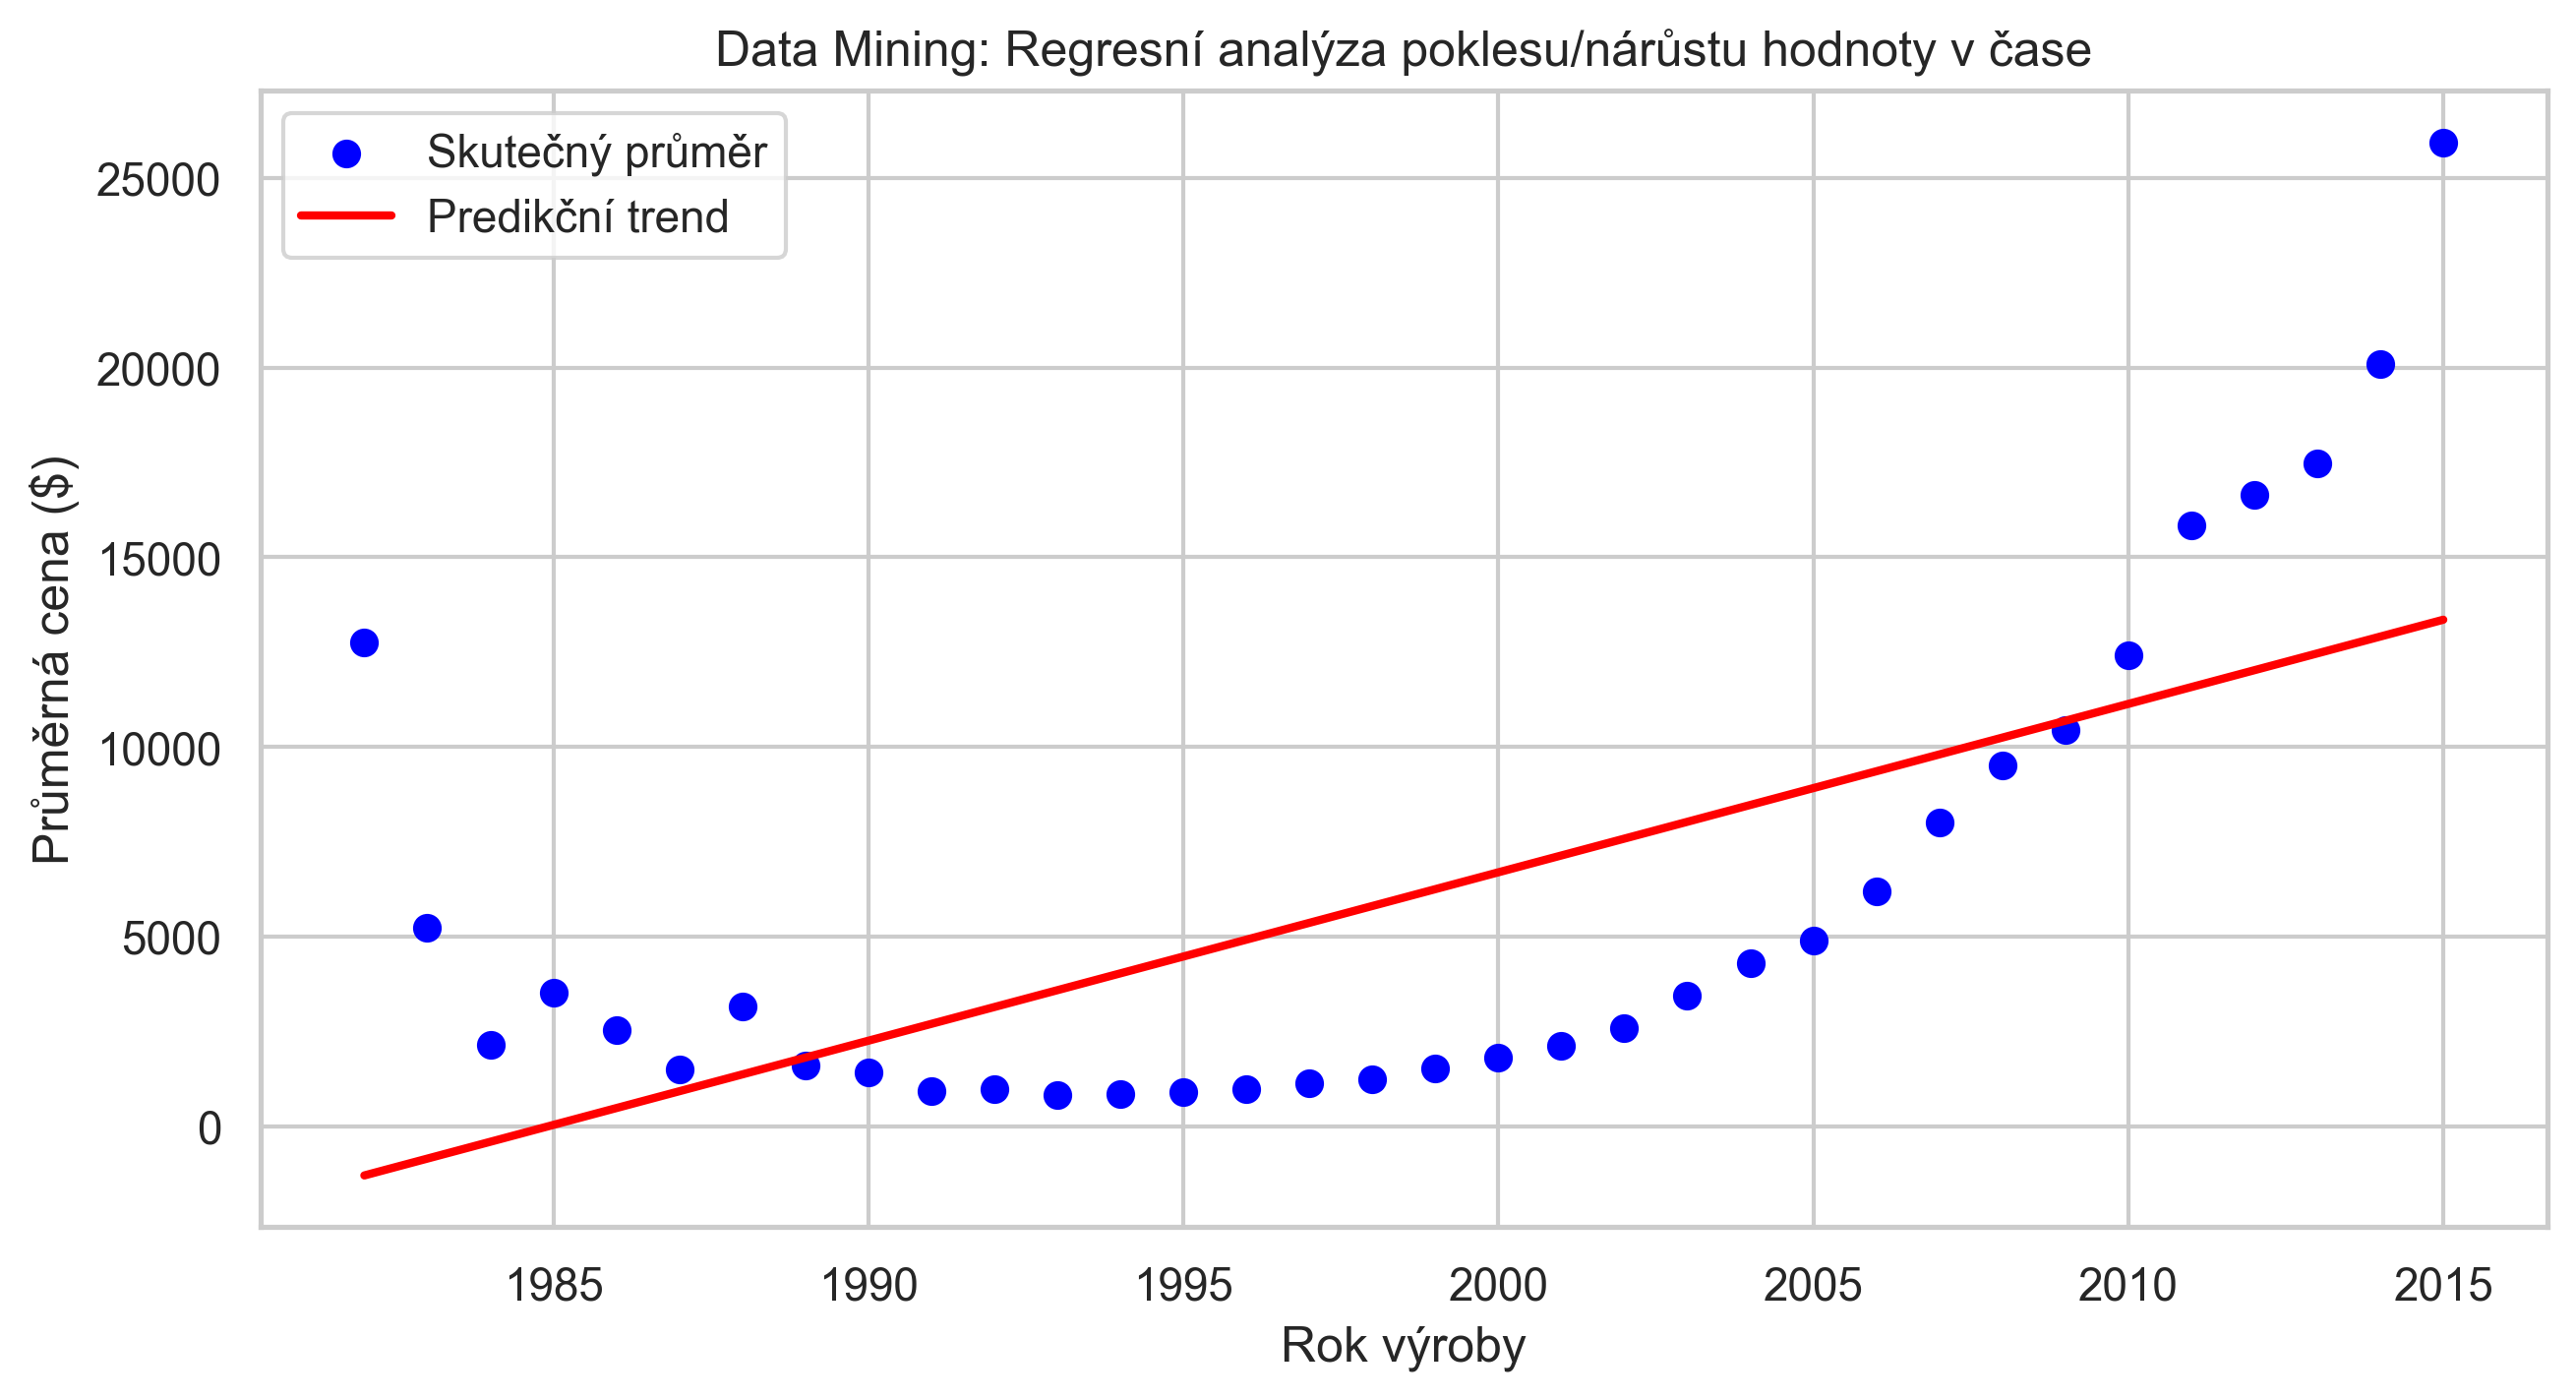
\includegraphics[width=0.8\textwidth]{../output/regression_trend.png}
%        \caption{Lineární regrese: Cena vs. Rok výroby}
%    \end{figure}

% V sekci "8. Data Mining - C. Anomálie":
%    \begin{figure}[H]
%        \centering
%        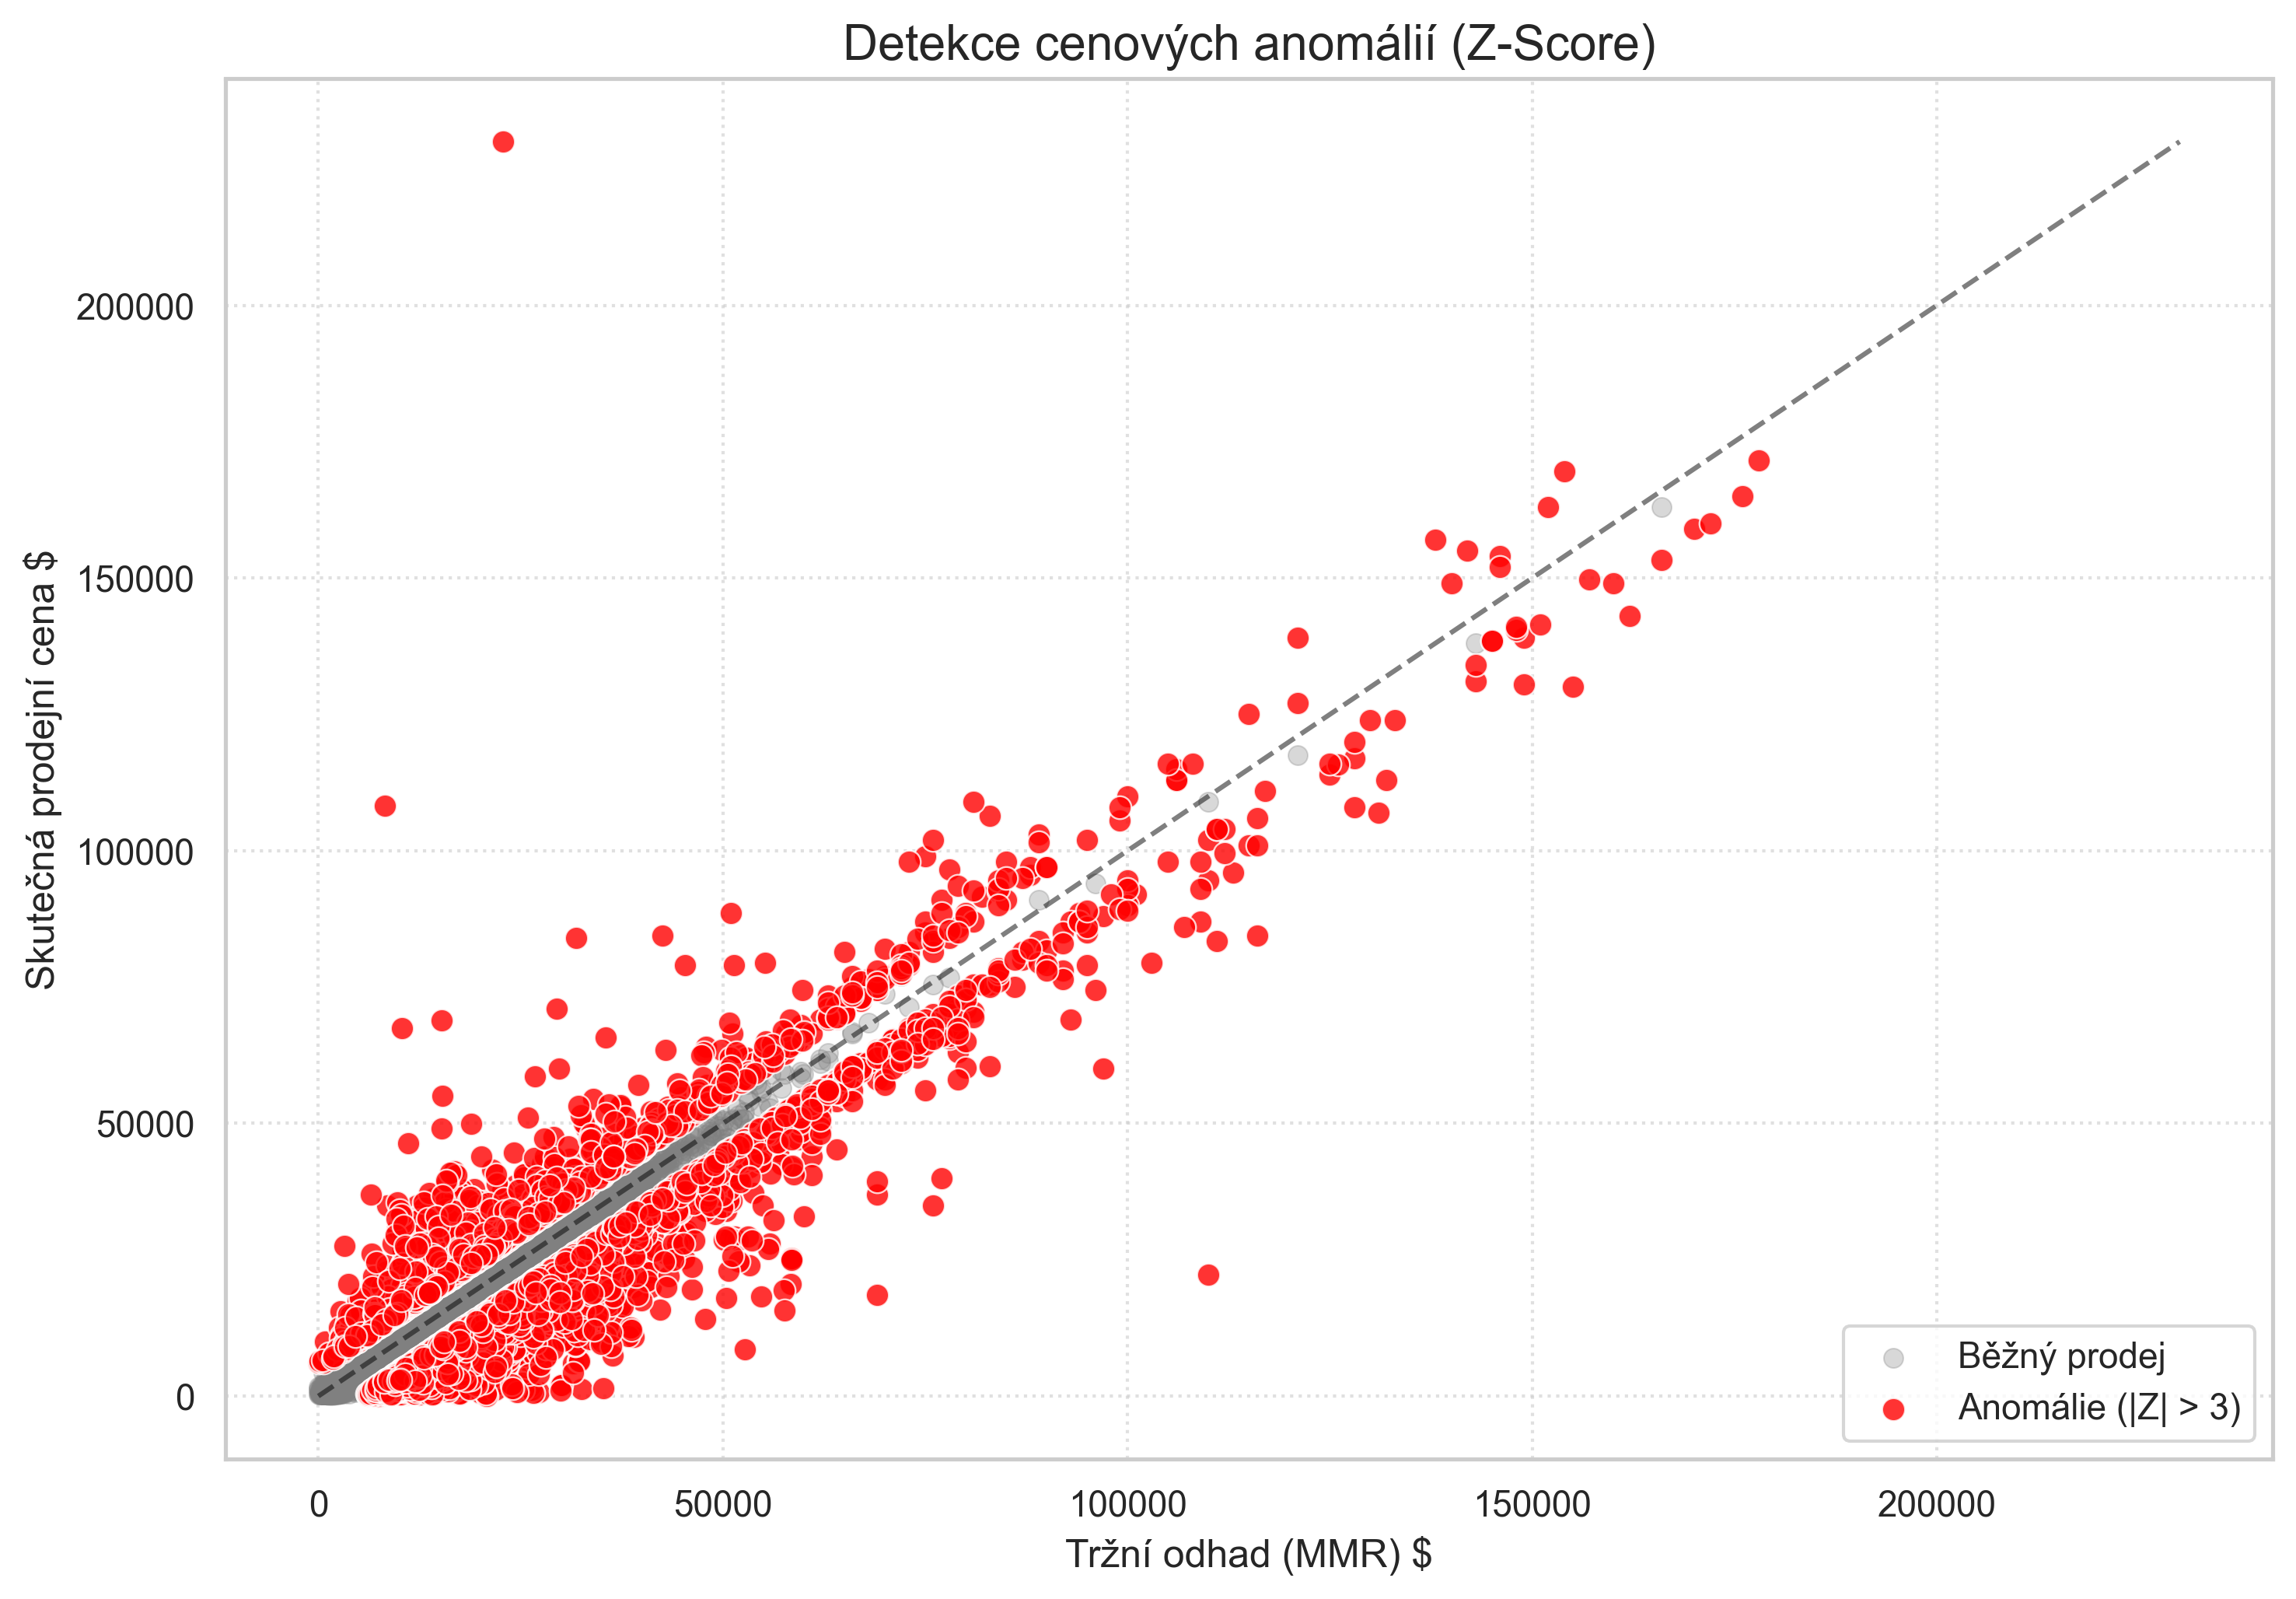
\includegraphics[width=0.8\textwidth]{../output/anomaly_detection.png}
%        \caption{Detekce anomálií: Skutečná cena vs. MMR}
%    \end{figure}

% ============================================================================
% SHRNUTÍ: SVŮ SI PAMATOVAT
% ============================================================================

% 1. Všechny \includegraphics musí ukazovat na reálné soubory!
% 2. Používej relativní cesty: ../output/   nebo   ./figures/
% 3. Podporované formáty: .png, .jpg, .pdf, .svg (pokud máš xetex)
% 4. [H] = umístit přesně sem, [t] = top, [b] = bottom, [p] = own page
% 5. width=0.85\textwidth = výchozí šírka (přizpůsob podle potřeby)
% 6. Vždy přidej \caption a \label pro referencování

% Kdyby něco nefungovalo, podívej se na error v PDF výstupu nebo zkus Overleaf debugging.
